% Options for packages loaded elsewhere
\PassOptionsToPackage{unicode}{hyperref}
\PassOptionsToPackage{hyphens}{url}
%
\documentclass[
]{article}
\title{XS3310 Teoría Estadística}
\usepackage{etoolbox}
\makeatletter
\providecommand{\subtitle}[1]{% add subtitle to \maketitle
  \apptocmd{\@title}{\par {\large #1 \par}}{}{}
}
\makeatother
\subtitle{I Semestre 2020}
\author{}
\date{\vspace{-2.5em}2021-06-07}

\usepackage{amsmath,amssymb}
\usepackage{lmodern}
\usepackage{iftex}
\ifPDFTeX
  \usepackage[T1]{fontenc}
  \usepackage[utf8]{inputenc}
  \usepackage{textcomp} % provide euro and other symbols
\else % if luatex or xetex
  \usepackage{unicode-math}
  \defaultfontfeatures{Scale=MatchLowercase}
  \defaultfontfeatures[\rmfamily]{Ligatures=TeX,Scale=1}
\fi
% Use upquote if available, for straight quotes in verbatim environments
\IfFileExists{upquote.sty}{\usepackage{upquote}}{}
\IfFileExists{microtype.sty}{% use microtype if available
  \usepackage[]{microtype}
  \UseMicrotypeSet[protrusion]{basicmath} % disable protrusion for tt fonts
}{}
\makeatletter
\@ifundefined{KOMAClassName}{% if non-KOMA class
  \IfFileExists{parskip.sty}{%
    \usepackage{parskip}
  }{% else
    \setlength{\parindent}{0pt}
    \setlength{\parskip}{6pt plus 2pt minus 1pt}}
}{% if KOMA class
  \KOMAoptions{parskip=half}}
\makeatother
\usepackage{xcolor}
\IfFileExists{xurl.sty}{\usepackage{xurl}}{} % add URL line breaks if available
\IfFileExists{bookmark.sty}{\usepackage{bookmark}}{\usepackage{hyperref}}
\hypersetup{
  pdftitle={XS3310 Teoría Estadística},
  hidelinks,
  pdfcreator={LaTeX via pandoc}}
\urlstyle{same} % disable monospaced font for URLs
\usepackage[margin=1in]{geometry}
\usepackage{graphicx}
\makeatletter
\def\maxwidth{\ifdim\Gin@nat@width>\linewidth\linewidth\else\Gin@nat@width\fi}
\def\maxheight{\ifdim\Gin@nat@height>\textheight\textheight\else\Gin@nat@height\fi}
\makeatother
% Scale images if necessary, so that they will not overflow the page
% margins by default, and it is still possible to overwrite the defaults
% using explicit options in \includegraphics[width, height, ...]{}
\setkeys{Gin}{width=\maxwidth,height=\maxheight,keepaspectratio}
% Set default figure placement to htbp
\makeatletter
\def\fps@figure{htbp}
\makeatother
\setlength{\emergencystretch}{3em} % prevent overfull lines
\providecommand{\tightlist}{%
  \setlength{\itemsep}{0pt}\setlength{\parskip}{0pt}}
\setcounter{secnumdepth}{-\maxdimen} % remove section numbering
\ifLuaTeX
  \usepackage{selnolig}  % disable illegal ligatures
\fi

\begin{document}
\maketitle

class: center, middle

\hypertarget{quuxe9-hemos-visto-hasta-ahora}{%
\section{¿Qué hemos visto hasta
ahora?}\label{quuxe9-hemos-visto-hasta-ahora}}

Todo sobre estimadores puntuales + pivotes e intervalos de confianza, IC
con bootstrap. Contrastes de hipótesis y + bootstrap.

\hypertarget{quuxe9-vamos-a-discutir-hoy}{%
\section{¿Qué vamos a discutir hoy?}\label{quuxe9-vamos-a-discutir-hoy}}

Un breve repaso de inferencia estadística para entender los errores
conceptuales más comunes.

\begin{center}\rule{0.5\linewidth}{0.5pt}\end{center}

\hypertarget{fisher-neyman-pearson-y-el-huxedbrido-nhst}{%
\section{Fisher, Neyman-Pearson, y el híbrido
NHST}\label{fisher-neyman-pearson-y-el-huxedbrido-nhst}}

\begin{itemize}
\item
  Los contrastes de hipótesis que se estudian en los cursos de carrera y
  de servicio, pueden ser controversiales.
\item
  La razón de esa controversia tiene que ver con las diferencias entre
  dos corrientes distintas dentro de la estadística clásica: Fisher vs
  Neyman-Pearson
\item
  Hoy vamos a repasar este artículo:
  \url{https://www.frontiersin.org/articles/10.3389/fpsyg.2015.00223/full}
  para aclarar algunas dudas acerca de lo que Uds han aprendido hasta
  ahora en la carrera de estadística.
\end{itemize}

\begin{center}\rule{0.5\linewidth}{0.5pt}\end{center}

\hypertarget{cronologuxeda}{%
\section{Cronología}\label{cronologuxeda}}

\begin{itemize}
\item
  Test de significancia: Fisher ayudó a desarrollarlo y lo promovió
  desde el año 1925.
\item
  Test de hipótesis estadísticas: desarrollado por Neyman y Pearson
  (1928)
\item
  Test de significancia de hipótesis nulas (NHST por sus siglas en
  inglés). Esta propuesta híbrida fue hecha por Lindquist (1940).
\item
  Estas dos corrientes (y un tercer híbrido) pertenecen a la estadística
  clásica, sin embargo, existen otras corrientes como el contraste de
  hipótesis de Bayes (Lindley, 1965) y la corriente de teoría de
  decisión de Wald (1950) que no se discutirán hoy.
\end{itemize}

\begin{center}\rule{0.5\linewidth}{0.5pt}\end{center}

\hypertarget{paruxe9ntesis}{%
\section{(Paréntesis)}\label{paruxe9ntesis}}

¿Por qué en estas semanas han están tratando de quitarle el nombre de
Fisher a un premio muy prestigioso?

Fisher era eugenista, lo que significa que era parte de un movimiento en
el estudio de la genética que abogaba por una raza superior. Los
estudios de ese grupo han sido muy cuestionados en la ciencia moderna,
por lo que, aunque los descrubrimientos de Fisher fueron seminales y muy
importantes para la estadística, la gente que pide el cambio de nombre
argumenta que no podemos glorificar a una persona racista, como Fisher.

Pueden leer más aquí:
\url{https://twitter.com/EKTBenn/status/1268869989785796610?s=20}

\begin{center}\rule{0.5\linewidth}{0.5pt}\end{center}

\hypertarget{la-propuesta-de-fisher}{%
\section{La propuesta de Fisher}\label{la-propuesta-de-fisher}}

\begin{itemize}
\item
  \emph{Paso 1:} seleccione una prueba adecuada.
\item
  \emph{Paso 2:} configure la hipótesis nula (H0) / Noten que solo es la
  hipótesis nula, no la alternativa.
\item
  \emph{Paso 3:} calcule la probabilidad teórica de los resultados bajo
  H0 - todo el procedimiento está basado en el supuesto de que la
  hipótesis nula es cierta.
\item
  \emph{Paso 4:} evalue la importancia estadística de los resultados -
  ¿el valor p es muy pequeño o muy grande? ¿cuál es el nivel de
  significancia? Corrección por pruebas múltiples.
\item
  \emph{Paso 5:} interprete la significación estadística de los
  resultados
\end{itemize}

\begin{center}\rule{0.5\linewidth}{0.5pt}\end{center}

\hypertarget{discusiuxf3n---fisher}{%
\section{Discusión - Fisher}\label{discusiuxf3n---fisher}}

\begin{itemize}
\item
  Dudar o negar la H0 dado un valor p bajo no necesariamente ``apoya'' o
  ``prueba'' que lo contrario es cierto.
\item
  Más importante aún, no ``apoya'' ni ``prueba'' que cualquier otra cosa
  que se haya hecho en la investigación tampoco explique los resultados
  (Macdonald, 1997).
\item
  Para Fisher, un buen control del diseño de la investigación (Fisher,
  1955; Johnstone, 1987; Cortina y Dunlap, 1997), especialmente la
  asignación aleatoria, es fundamental para hacer inferencias razonables
  basadas en los resultados de las pruebas de significancia (Fisher,
  1954; Neyman , 1967).
\item
  Finalmente, consideró los resultados significativos como meros puntos
  de datos y alentó el uso del metanálisis para avanzar más, combinando
  resultados significativos y no significativos de proyectos de
  investigación relacionados (Fisher, 1960; Neyman, 1967).
\end{itemize}

\begin{center}\rule{0.5\linewidth}{0.5pt}\end{center}

\hypertarget{puntos-destacados---fisher}{%
\section{Puntos destacados (+) -
Fisher}\label{puntos-destacados---fisher}}

\begin{itemize}
\item
  Flexibilidad. Debido a que la mayor parte del trabajo se realiza a
  posteriori, el enfoque de Fisher es bastante flexible, lo que permite
  llevar a cabo cualquier cantidad de pruebas.
\item
  Más adecuado para proyectos de investigación ad-hoc o estudios
  explotarios.
\item
  Inferencial. El procedimiento de Fisher es en gran medida inferencial,
  desde la muestra hasta la población de referencia, aunque de alcance
  limitado, principalmente restringido a poblaciones que comparten
  parámetros similares a los estimados a partir de la muestra (Fisher,
  1954, 1955; Macdonald, 2002; Hubbard, 2004).
\end{itemize}

\begin{center}\rule{0.5\linewidth}{0.5pt}\end{center}

\hypertarget{puntos-destacados-----fisher}{%
\section{Puntos destacados (-) -
Fisher}\label{puntos-destacados-----fisher}}

\begin{itemize}
\item
  Sin análisis de potencia. Fisher habló de sensibilidad de la prueba,
  sin embargo, nunca creó un procedimiento matemático para controlar la
  sensibilidad de una manera predecible (Macdonald, 1997; Hubbard,
  2004).
\item
  No hay hipótesis alternativa. Fisher consideró implícitamente
  hipótesis alternativas, que son la negación de las hipótesis nulas,
  tanto que para él la tarea principal del investigador, y la definición
  de un proyecto de investigación bien hecho, fue rechazar
  sistemáticamente con suficiente evidencia el nulo correspondiente.
\end{itemize}

\begin{center}\rule{0.5\linewidth}{0.5pt}\end{center}

\hypertarget{la-propuesta-de-neyman-pearson}{%
\section{La propuesta de
Neyman-Pearson}\label{la-propuesta-de-neyman-pearson}}

A priori:

\begin{itemize}
\item
  \emph{Paso 1:} configure el tamaño del efecto esperado en la
  población.
\item
  \emph{Paso 2:} seleccione una prueba óptima.
\item
  \emph{Paso 3:} configure la hipótesis principal (HM). Error tipo I.
  Alfa (α). La región crítica (CRtest) y el valor crítico (CVtest,
  Testcrit) de una prueba.
\item
  \emph{Paso 4:} configure la hipótesis alternativa (HA). Error tipo II
  Beta (β).
\item
  \emph{Paso 5:} calcule el tamaño de muestra (N) requerido para una
  buena potencia (1 -- β)
\item
  \emph{Paso 6:} calcule el valor crítico de la prueba.
\end{itemize}

\begin{center}\rule{0.5\linewidth}{0.5pt}\end{center}

\hypertarget{la-propuesta-de-neyman-pearson-1}{%
\section{La propuesta de
Neyman-Pearson}\label{la-propuesta-de-neyman-pearson-1}}

A posteriori:

\begin{itemize}
\item
  \emph{Paso 7:} calcule el valor de la prueba para la investigación
  (RVtest).
\item
  \emph{Paso 8} decida a favor de la hipótesis principal o alternativa.
\end{itemize}

\begin{center}\rule{0.5\linewidth}{0.5pt}\end{center}

\hypertarget{discusiuxf3n---neyman-pearson}{%
\section{Discusión -
Neyman-Pearson}\label{discusiuxf3n---neyman-pearson}}

\begin{itemize}
\item
  El enfoque de Neyman-Pearson lleva a una decisión entre hipótesis
  (Neyman y Pearson, 1933; Spielman, 1978). En la práctica, realmente no
  hace mucha diferencia si acepta HM o HA, según corresponda (Macdonald,
  1997). De hecho, aceptar HM o HA es beneficioso ya que evita la
  confusión con el enfoque de Fisher, que solo puede rechazar H0
  (Perezgonzalez, 2014).
\item
  Informar el valor de la prueba de investigación observada es relevante
  bajo el enfoque de Neyman-Pearson, ya que sirve para comparar el valor
  observado con el valor crítico a priori.
\item
  También se supone que las hipótesis de Neyman-Pearson son ciertas.
  Esto significa que HM y HA no pueden ser, al mismo tiempo, falsas, ni
  demostrarse o falsificarse a posteriori. El único camino a seguir es
  actuar como si la conclusión a la que llegara la prueba fuera cierta,
  sujeto a una probabilidad α o β de cometer un error de Tipo I o Tipo
  II, respectivamente (Neyman y Pearson, 1933; Cortina y Dunlap, 1997).
\end{itemize}

\begin{center}\rule{0.5\linewidth}{0.5pt}\end{center}

\hypertarget{puntos-destacados---neyman-pearson}{%
\section{Puntos destacados (+) -
Neyman-Pearson}\label{puntos-destacados---neyman-pearson}}

\begin{itemize}
\item
  Mejor potencia. El enfoque de Neyman-Pearson es más poderoso que el de
  Fisher para probar datos a largo plazo (Williams et al., 2006).
\item
  Más adecuado para proyectos de muestreo repetido. Utilizando la misma
  población y pruebas, como el control de calidad industrial o las
  pruebas de diagnóstico a gran escala (Fisher, 1955; Spielman, 1973).
\item
  Deductivo. El enfoque es deductivo y bastante mecánico una vez que se
  han establecido los pasos a priori (Neyman y Pearson, 1933; Neyman,
  1942; Fisher, 1955).
\end{itemize}

\begin{center}\rule{0.5\linewidth}{0.5pt}\end{center}

\hypertarget{puntos-destacados-----neyman-pearson}{%
\section{Puntos destacados (-) -
Neyman-Pearson}\label{puntos-destacados-----neyman-pearson}}

\begin{itemize}
\item
  Menos flexible que el enfoque de Fisher. Debido a que la mayor parte
  del trabajo se realiza a priori, este enfoque es menos flexible para
  acomodar pruebas no pensadas de antemano y para realizar
  investigaciones exploratorias (Macdonald, 2002).
\item
  Por defecto se adapta fácilmente al enfoque de Fisher. Como este
  enfoque parece superficialmente similar al de Fisher, es fácil
  confundir ambos y olvidar lo que hace que el enfoque de Neyman-Pearson
  sea único (Lehman, 1993). Si la información proporcionada por la
  hipótesis alternativa (ES y β) no se tiene en cuenta para diseñar una
  investigación con buena potencia, el análisis de datos se basa en la
  prueba de significancia de Fisher.
\end{itemize}

\begin{center}\rule{0.5\linewidth}{0.5pt}\end{center}

\hypertarget{nhst---el-muxe9todo-huxedbrido}{%
\section{NHST - el método
híbrido}\label{nhst---el-muxe9todo-huxedbrido}}

\begin{itemize}
\item
  El NHST es el procedimiento más común utilizado para probar datos hoy
  en día, aunque bajo el supuesto falso de probar hipótesis sustantivas
  (Carver, 1978; Nickerson, 2000; Hubbard, 2004; Hager, 2013).
\item
  NHST es, en realidad, una amalgama de las teorías de Fisher y
  Neyman-Pearson, que se ofrece como un enfoque continuo para las
  pruebas (Macdonald, 2002; Gigerenzer, 2004). Tampoco es una
  amalgamación claramente definida y, dependiendo del autor que lo
  describa o del investigador que la use, puede desviarse más hacia el
  enfoque de Fisher o hacia el enfoque de Neyman-Pearson.
\item
  Desafortunadamente, si comparamos los enfoques de Fisher y
  Neyman-Pearson frente a frente, encontramos que son incompatibles en
  la mayoría de las cuentas (ver tabla en la siguiente filmina).
\item
  Sin embargo, en general, la mayoría de las amalgamaciones siguen a
  Neyman-Pearson de manera procesal pero a Fisher filosóficamente
  (Spielman, 1978; Johnstone, 1986; Cortina y Dunlap, 1997; Hubbard,
  2004).
\end{itemize}

\begin{center}\rule{0.5\linewidth}{0.5pt}\end{center}

\hypertarget{tabla-comparativa}{%
\section{Tabla comparativa}\label{tabla-comparativa}}

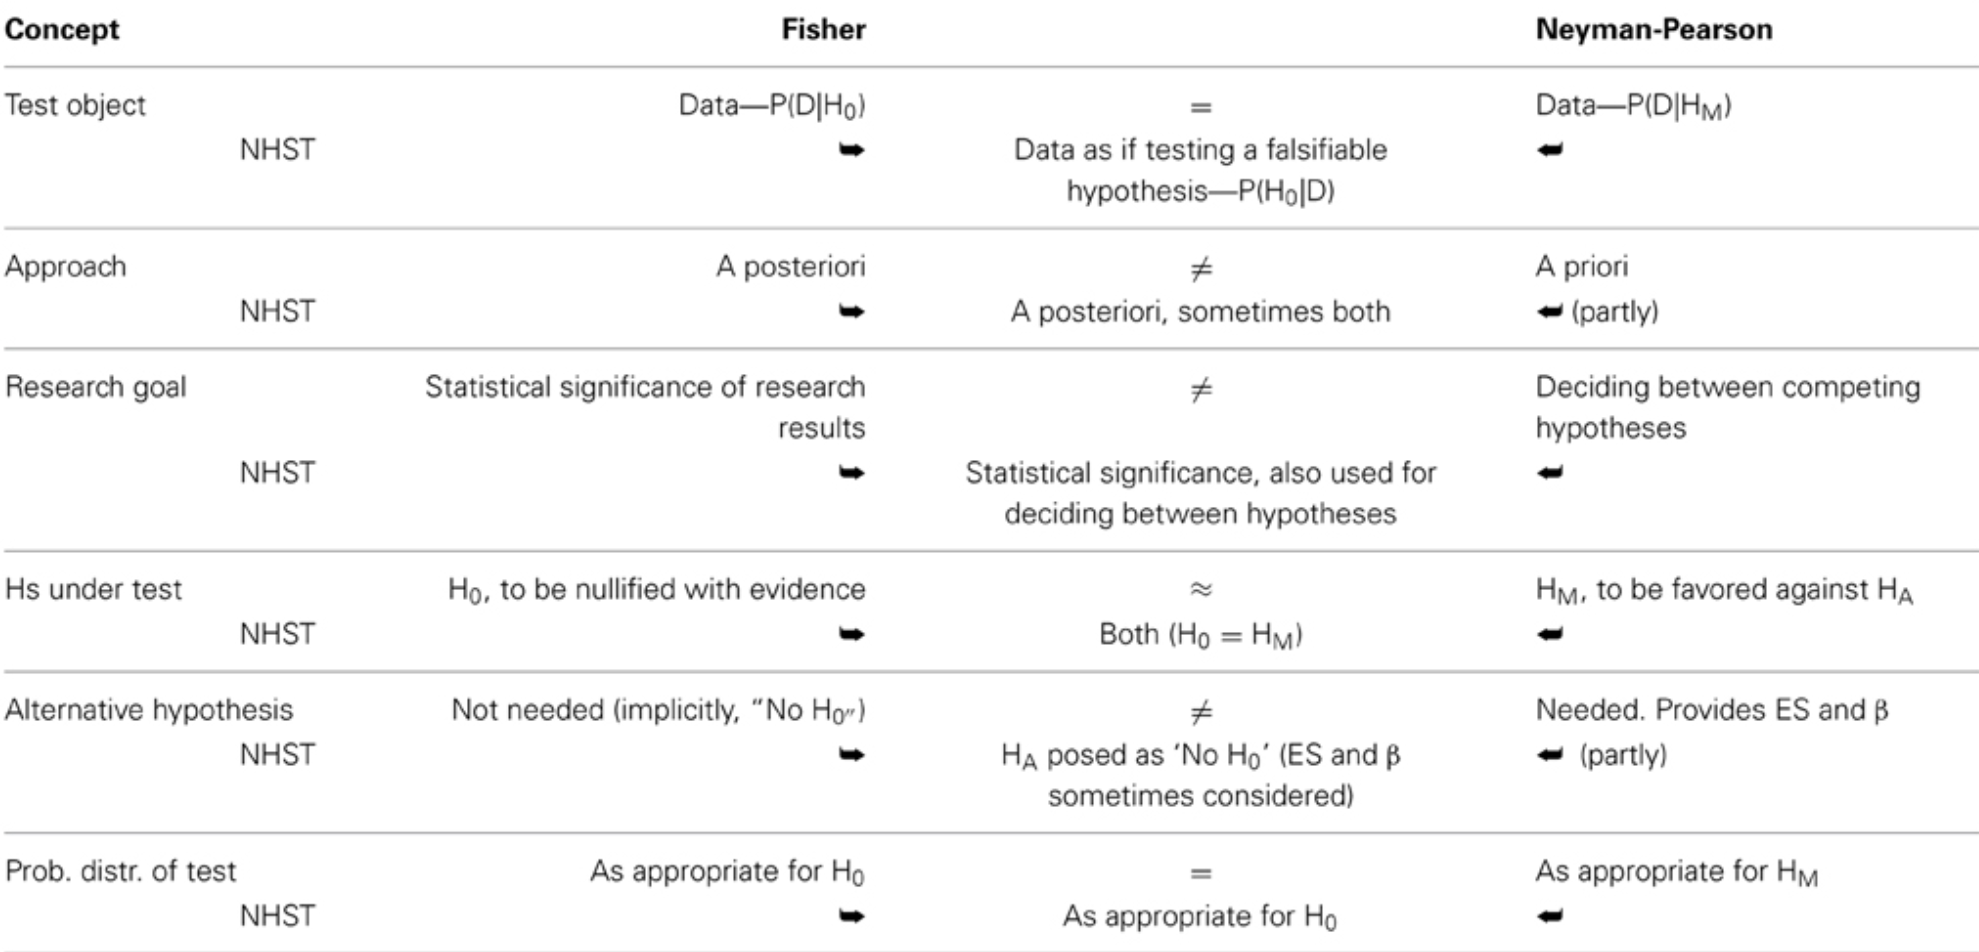
\includegraphics{figs/tabla1.1.png} Fuente:
\url{https://www.frontiersin.org/files/Articles/135153/fpsyg-06-00223-HTML/image_m/fpsyg-06-00223-t001.jpg}

\begin{center}\rule{0.5\linewidth}{0.5pt}\end{center}

\hypertarget{tabla-comparativa-continuaciuxf3n}{%
\section{Tabla comparativa
(continuación)}\label{tabla-comparativa-continuaciuxf3n}}

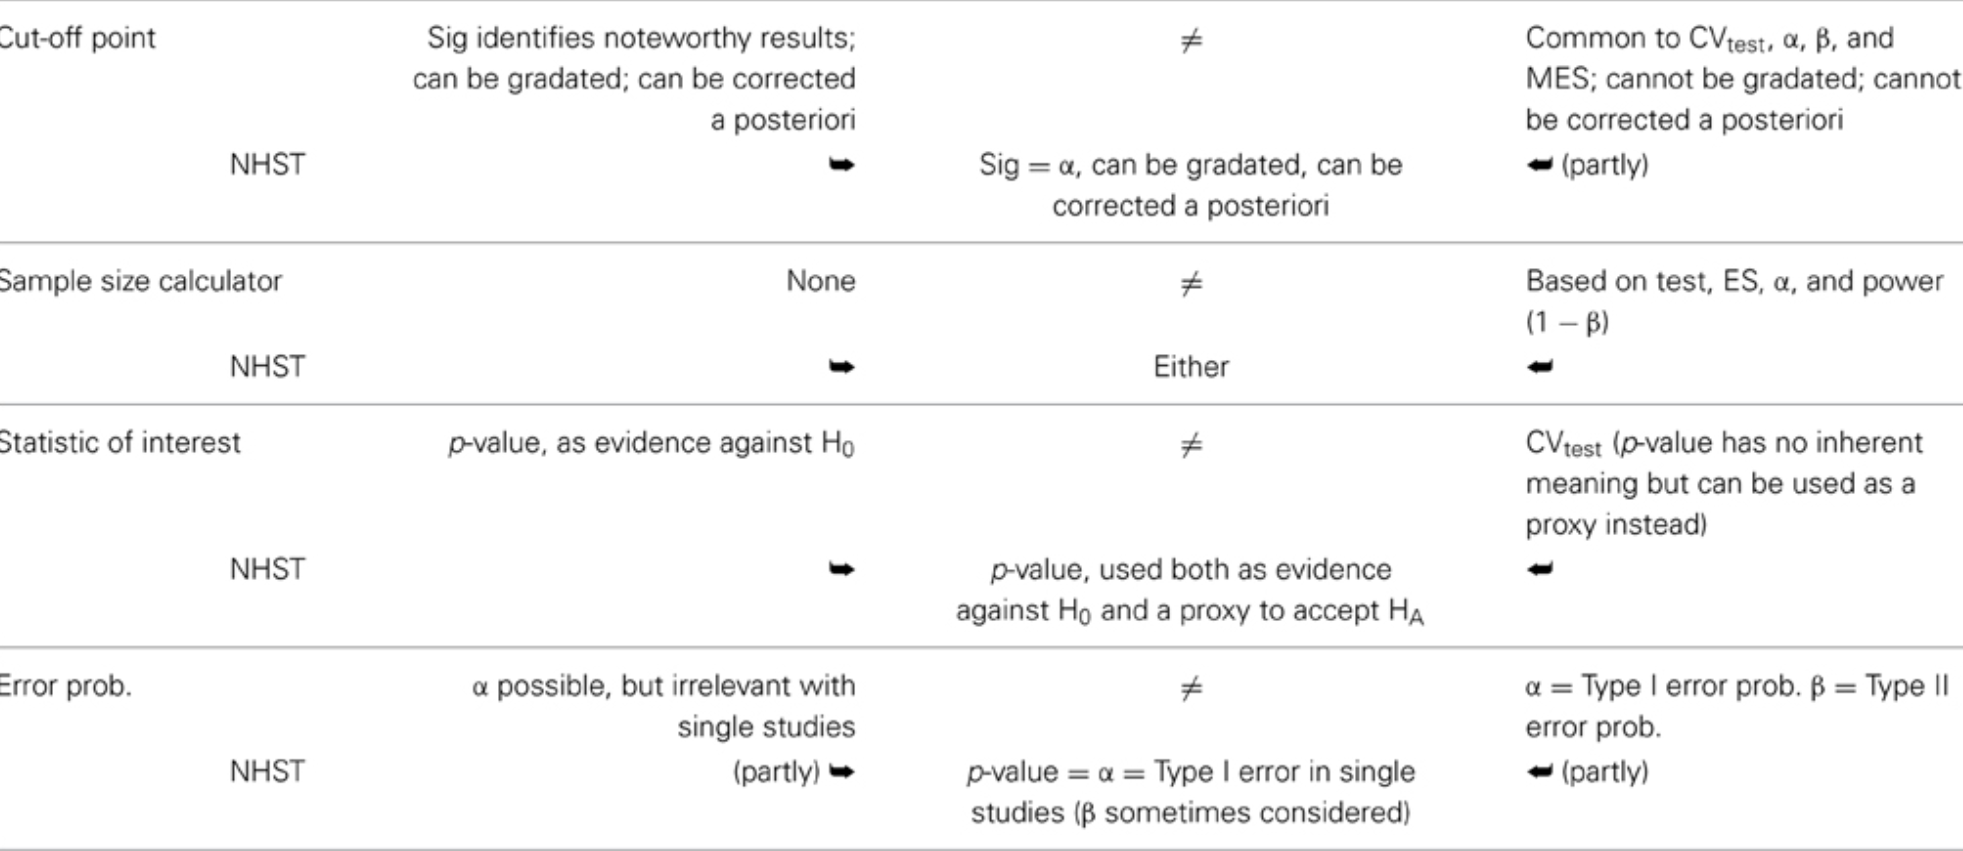
\includegraphics{figs/tabla1.2.png}

\hypertarget{fuente-httpswww.frontiersin.orgfilesarticles135153fpsyg-06-00223-htmlimage_mfpsyg-06-00223-t001.jpg}{%
\subsection{\texorpdfstring{Fuente:
\url{https://www.frontiersin.org/files/Articles/135153/fpsyg-06-00223-HTML/image_m/fpsyg-06-00223-t001.jpg}}{Fuente: https://www.frontiersin.org/files/Articles/135153/fpsyg-06-00223-HTML/image\_m/fpsyg-06-00223-t001.jpg}}\label{fuente-httpswww.frontiersin.orgfilesarticles135153fpsyg-06-00223-htmlimage_mfpsyg-06-00223-t001.jpg}}

\hypertarget{tabla-comparativa-continuaciuxf3n-1}{%
\section{Tabla comparativa
(continuación)}\label{tabla-comparativa-continuaciuxf3n-1}}

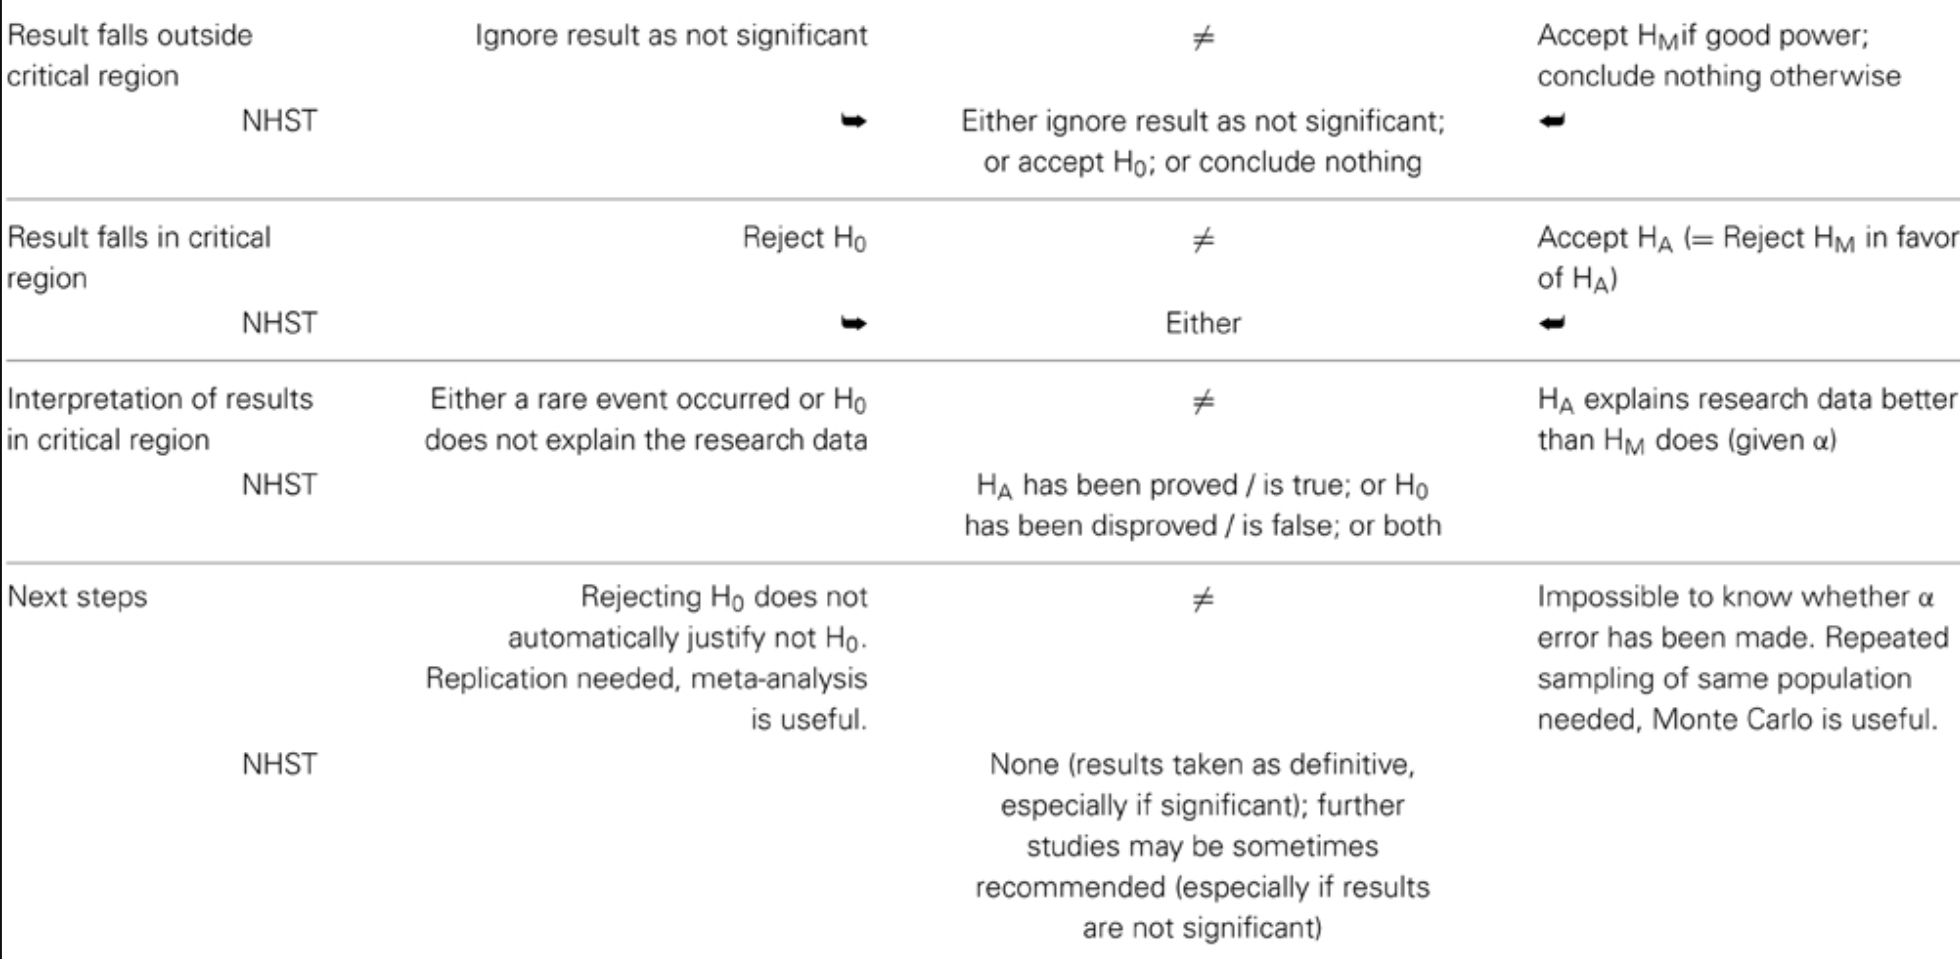
\includegraphics{figs/tabla1.3.png}

\hypertarget{fuente-httpswww.frontiersin.orgfilesarticles135153fpsyg-06-00223-htmlimage_mfpsyg-06-00223-t001.jpg-1}{%
\subsection{\texorpdfstring{Fuente:
\url{https://www.frontiersin.org/files/Articles/135153/fpsyg-06-00223-HTML/image_m/fpsyg-06-00223-t001.jpg}}{Fuente: https://www.frontiersin.org/files/Articles/135153/fpsyg-06-00223-HTML/image\_m/fpsyg-06-00223-t001.jpg}}\label{fuente-httpswww.frontiersin.orgfilesarticles135153fpsyg-06-00223-htmlimage_mfpsyg-06-00223-t001.jpg-1}}

\hypertarget{ejercicio-para-pensar}{%
\section{Ejercicio para pensar}\label{ejercicio-para-pensar}}

\begin{itemize}
\item
  Hagan una lista de los cursos que han llevado de la carrera de
  estadística. Identifiquen en cuáles cursos han usado los conceptos de
  cada tendencia: Fisher, Neyman-Pearson y/o NHST.
\item
  Otros ejercicios:
\item
  Práctica de contrastes (para hacerla en sus casas):
  \url{http://math.arizona.edu/~jwatkins/r-composite.pdf}
\item
  Tarea moral en Mediación Virtual (Potencia de dos contrastes de
  hipótesis para la diferencia de mediasArchivo).
\end{itemize}

\begin{center}\rule{0.5\linewidth}{0.5pt}\end{center}

class: center, middle

\hypertarget{quuxe9-discutimos-hoy}{%
\section{¿Qué discutimos hoy?}\label{quuxe9-discutimos-hoy}}

Repaso de la inferencia clásica, específicamente las pruebas de
hipótesis.

\hypertarget{quuxe9-nos-falta-para-el-ii-parcial}{%
\section{¿Qué nos falta para el II
Parcial?}\label{quuxe9-nos-falta-para-el-ii-parcial}}

Discusión de ensayos de valores p.

Slides creadas via R package
\href{https://github.com/yihui/xaringan}{\textbf{xaringan}}.

\end{document}
